% ------------------------------------------------------------------------------
% Este fichero es parte de la plantilla LaTeX para la realización de Proyectos
% Final de Grado, protegido bajo los términos de la licencia GFDL.
% Para más información, la licencia completa viene incluida en el
% fichero fdl-1.3.tex

% Copyright (C) 2012 SPI-FM. Universidad de Cádiz
% ------------------------------------------------------------------------------

\section{Catálogo de actores}
Los usuarios que interactúan con el sistema se diferencian en actores, en este caso, dietista, paciente y administrador.
\begin{itemize}
\item \textbf{Dietista:} Este actor será el responsable directo de la interactuación con la aplicación, siendo responsable de todos los requisitos funcionales.
\item \textbf{Paciente:} Este actor intervendrá en algunos de los requisitos y será el mayor beneficiario de la aplicación.
\item \textbf{Administrador:} Este actor sólo intervendrá en el caso de uso \textit{Eliminar Perfil Dietista}, siendo necesario para poder llevarse a cabo la acción.
\end{itemize}

\section{Requisitos funcionales}
A continuación se exponen los requisitos funcionales de la aplicación:
\begin{itemize}
\item \textbf{Requisitos funcionales de la gestión de dietistas:}
\begin{itemize}
\item Se podrá añadir un nuevo dietista a la aplicación registrando sus propios datos.
\item Se podrá abrir un perfil de dietista existente, previamente registrado, y suministrando la clave correspondiente.
\item Se podrá cerrar un perfil de dietista abierto previamente.
\item Se podrá eliminar un perfil de dietista existente.
\end{itemize}
\item \textbf{Requisitos funcionales de la gestión de pacientes:}
\begin{itemize}
\item Se podrá añadir un nuevo paciente a la aplicación, registrando el dietista los datos de dicho paciente.
\item Se podrá abrir un perfil de paciente existente y perteneciente al dietista actualmente en uso de la aplicación.
\item Se podrán editar los datos de un perfil de paciente una vez abierto mediante el botón guardar.
\item Se podrá cerrar un perfil de paciente abierto previamente.
\item Se podrá eliminar un perfil de paciente existente y perteneciente al dietista actualmente en uso de la aplicación.
\item Se podrá añadir y modificar información médica referente al paciente, tales como analíticas, tratamiento farmacológico o enfermedades/patologías.
\item Se podrá añadir información general referente al paciente.
\item Se podrán añadir diarios dietéticos rellenados por el paciente.
\item Se podrán eliminar diarios dietéticos de un paciente.
\item Se podrán añadir recordatorios 24h. rellenados por el paciente.
\item Se podrán eliminar recordatorios 24h. de un paciente.
\item Se podrá añadir la frecuencia de ingesta de alimentos de un paciente.
\item Se podrán añadir recetas al semanario del paciente en uso.
\item Se podrán ver los semanarios existentes del paciente en uso.
\end{itemize}
\item \textbf{Requisitos funcionales de la gestión de recetas:}
\begin{itemize}
\item Se podrán añadir nuevas recetas de un dietista en uso.
\item Se podrán editar recetas existentes de un dietista en uso.
\item Se podrán eliminar recetas existentes de un dietista en uso.
\end{itemize}
\end{itemize}

\section{Análisis}
\subsection{Modelos de casos de uso}
A continuación se muestran las especificaciones de casos de uso, con sus respectivos diagramas.
\subsubsection{Casos de uso respecto a la gestión de dietistas}
\begin{figure}[H]
  \label{cu_dietista}
  \begin{center}
    % Comentar si no está el paquete tkiz instalado, y descomentar la
    % linea siguiente. Comentar además la inclusión del paquete en
    % estilos/estiloBase.sty
    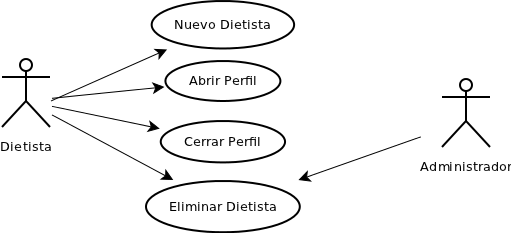
\includegraphics[scale=0.7]{../img/CU_Dietista.png}
  \end{center}
  \caption{Diagrama de caso de uso: Gestión de dietistas}
\end{figure}

\textbf{Caso de Uso: Nuevo Dietista}
\begin{itemize}
\item \textbf{Descripción:} Resgistro de dietista en el sistema.
\item \textbf{Precondición:} El dietista no existe en el sistema.
\item \textbf{Postcondición:} El dietista se registra en el sistema.
\item \textbf{Actores:} Dietista(principal)
\item \textbf{Resumen:} El dietista desea darse de alta en el sistema.
\item \textbf{Escenario Principal:}
\begin{enumerate}
\item El dietista solicita al sistema darse de alta.
\item El dietista rellena los datos solicitados.
\item El sistema comprueba los datos introducidos.
\item Se almacenan los datos en el sistema.
\end{enumerate}
\item \textbf{Escenario Alternativo:}
\begin{enumerate}
\item[0] En cualquier momento el dietista puede cancelar el proceso.
\item[3] Existen campos vacíos o erróneos. Mensajes de advertencia sobre los campos afectados.
\item[3a] Existe un dietista con el mismo DNI. Mensaje de advertencia del sistema.
\end{enumerate}
\end{itemize}
\begin{figure}[H]
  \label{ds_nuevodietista}
  \begin{center}
    % Comentar si no está el paquete tkiz instalado, y descomentar la
    % linea siguiente. Comentar además la inclusión del paquete en
    % estilos/estiloBase.sty
    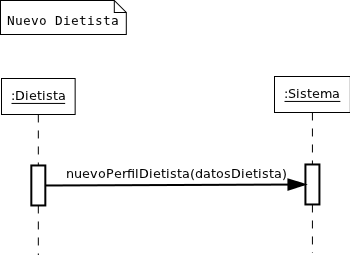
\includegraphics[scale=0.7]{../img/DS_NuevoDietista.png}
  \end{center}
  \caption{Diagrama de secuencia: Nuevo Dietista}
\end{figure}
\textbf{Contrato de la operación:} nuevoPerfilDietista(datosDietista)
\begin{itemize}
\item \textbf{Responsabilidades:} Registrar un nuevo dietista en el sistema.
\item \textbf{Referencias cruzadas:} Caso de uso ``Nuevo Dietista''.
\item \textbf{Precondición:}
\begin{itemize}
\item El dietista no se encuentra registrado en el sistema.
\item datosDietista es válido.
\end{itemize}
\item \textbf{Postcondición:}
\begin{itemize}
\item El dietista se guarda en el sistema.
\end{itemize}
\end{itemize}

\textbf{Caso de Uso: Abrir Perfil}
\begin{itemize}
\item \textbf{Descripción:} Abrir perfil de dietista solicitado.
\item \textbf{Precondición:} El dietista existe en el sistema.
\item \textbf{Postcondición:} El dietista abre perfil en el sistema.
\item \textbf{Actores:} Dietista(principal)
\item \textbf{Resumen:} El dietista desea abrir su perfil en el sistema.
\item \textbf{Escenario Principal:}
\begin{enumerate}
\item El dietista solicita al sistema abrir su perfil.
\item El dietista rellena la clave que se le solicita.
\item El sistema comprueba la clave introducida.
\item Se abre el perfil del dietista en el sistema.
\end{enumerate}
\item \textbf{Escenario Alternativo:}
\begin{enumerate}
\item[0] En cualquier momento el dietista puede cancelar el proceso.
\item[3] La clave es errónea. Mensaje de advertencia del sistema.
\end{enumerate}
\end{itemize}
\begin{figure}[H]
  \label{ds_abrirdietista}
  \begin{center}
    % Comentar si no está el paquete tkiz instalado, y descomentar la
    % linea siguiente. Comentar además la inclusión del paquete en
    % estilos/estiloBase.sty
    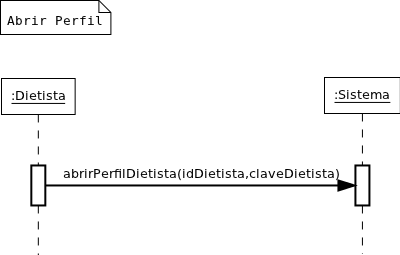
\includegraphics[scale=0.7]{../img/DS_AbrirDietista.png}
  \end{center}
  \caption{Diagrama de secuencia: Abrir Perfil Dietista}
\end{figure}
\textbf{Contrato de la operación:} abrirPerfilDietista(idDietista,claveDietista)
\begin{itemize}
\item \textbf{Responsabilidades:} Abrir perfil de dietista en el sistema.
\item \textbf{Referencias cruzadas:} Caso de uso ``Abrir Perfil''.
\item \textbf{Precondición:}
\begin{itemize}
\item Existe un dietista con id = idDietista.
\item claveDietista es válida.
\end{itemize}
\item \textbf{Postcondición:}
\begin{itemize}
\item El sistema carga los datos del dietista en el sistema.
\end{itemize}
\end{itemize}

\textbf{Caso de Uso: Cerrar Perfil}
\begin{itemize}
\item \textbf{Descripción:} Cerrar perfil de dietista en uso del sistema.
\item \textbf{Precondición:} El dietista tiene abierto su perfil en el sistema.
\item \textbf{Postcondición:} El dietista cierra su perfil en el sistema.
\item \textbf{Actores:} Dietista(principal)
\item \textbf{Resumen:} El dietista desea cerrar su perfil en el sistema.
\item \textbf{Escenario Principal:}
\begin{enumerate}
\item El dietista solicita al sistema cerrar su perfil.
\item El sistema cierra el perfil del dietista.
\item Se cierra el perfil del dietista en el sistema.
\end{enumerate}
\item \textbf{Escenario Alternativo:}
\begin{enumerate}
\item[0] En cualquier momento el dietista puede cancelar el proceso.
\end{enumerate}
\end{itemize}
\begin{figure}[H]
  \label{ds_cerrardietista}
  \begin{center}
    % Comentar si no está el paquete tkiz instalado, y descomentar la
    % linea siguiente. Comentar además la inclusión del paquete en
    % estilos/estiloBase.sty
    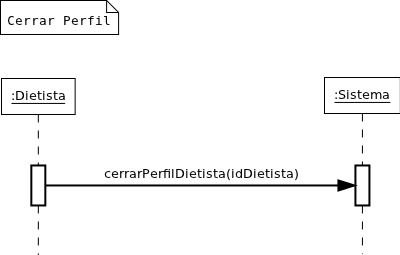
\includegraphics[scale=0.7]{../img/DS_CerrarDietista.png}
  \end{center}
  \caption{Diagrama de secuencia: Cerrar Perfil Dietista}
\end{figure}
\textbf{Contrato de la operación:} cerrarPerfilDietista(idDietista)
\begin{itemize}
\item \textbf{Responsabilidades:} Cerrar perfil de dietista en el sistema.
\item \textbf{Referencias cruzadas:} Caso de uso ``Cerrar Perfil''.
\item \textbf{Precondición:}
\begin{itemize}
\item Existe un Dietista D con D.id = idDiestista en uso.
\end{itemize}
\item \textbf{Postcondición:}
\begin{itemize}
\item El sistema cierra el perfil del dietista en el sistema.
\end{itemize}
\end{itemize}

\textbf{Caso de Uso: Eliminar Dietista}
\begin{itemize}
\item \textbf{Descripción:} Eliminar perfil de dietista del sistema.
\item \textbf{Precondición:} El dietista existe y no tiene abierto su perfil en el sistema.
\item \textbf{Postcondición:} El dietista elimina su perfil del sistema.
\item \textbf{Actores:} Dietista(principal) y Administrador(secundario)
\item \textbf{Resumen:} El dietista desea eliminar su perfil del sistema.
\item \textbf{Escenario Principal:}
\begin{enumerate}
\item El dietista solicita al sistema eliminar su perfil.
\item El dietista solicita al administrador la clave de confirmación y la introduce.
\item El sistema comprueba la clave de confimación.
\item Se elimina el perfil del dietista del sistema.
\end{enumerate}
\item \textbf{Escenario Alternativo:}
\begin{enumerate}
\item[0] En cualquier momento el dietista puede cancelar el proceso.
\item[3] La clave de confirmación es errónea. Mensaje de advertencia del sistema.
\end{enumerate}
\end{itemize}
\begin{figure}[H]
  \label{ds_eliminardietista}
  \begin{center}
    % Comentar si no está el paquete tkiz instalado, y descomentar la
    % linea siguiente. Comentar además la inclusión del paquete en
    % estilos/estiloBase.sty
    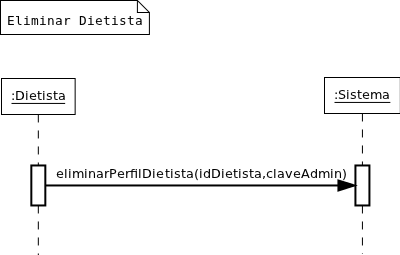
\includegraphics[scale=0.7]{../img/DS_EliminarDietista.png}
  \end{center}
  \caption{Diagrama de secuencia: Eliminar Dietista}
\end{figure}
\textbf{Contrato de la operación:} eliminarPerfilDietista(idDiestista, claveAdmin)
\begin{itemize}
\item \textbf{Responsabilidades:} Eliminar perfil de dietista del sistema.
\item \textbf{Referencias cruzadas:} Caso de uso ``Eliminar Dietista''.
\item \textbf{Precondición:}
\begin{itemize}
\item Existe un dietista con id = idDietista.
\item claveAdmin es válido.
\end{itemize}
\item \textbf{Postcondición:}
\begin{itemize}
\item Se eliminan los datos del dietista con idDietista.
\end{itemize}
\end{itemize}


\newpage
\subsubsection{Casos de uso respecto a la gestión de pacientes}
\begin{figure}[H]
  \label{cu_paciente}
  \begin{center}
    % Comentar si no está el paquete tkiz instalado, y descomentar la
    % linea siguiente. Comentar además la inclusión del paquete en
    % estilos/estiloBase.sty
    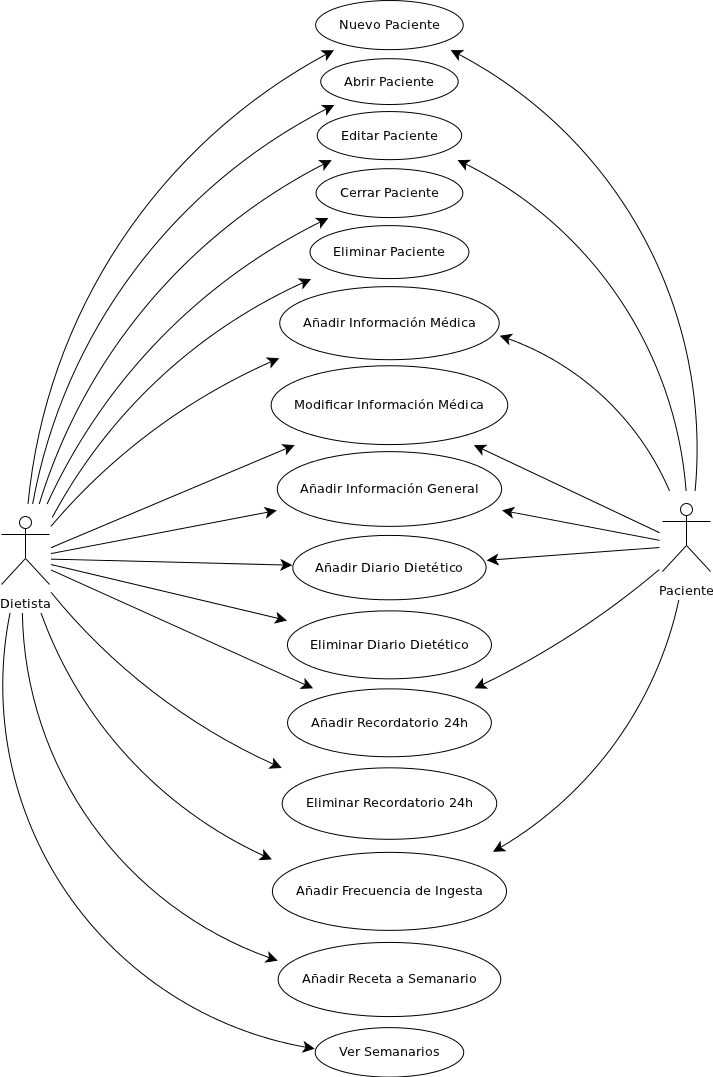
\includegraphics[scale=0.6]{../img/CU_Paciente.png}
  \end{center}
  \caption{Diagrama de caso de uso: Gestión de pacientes}
\end{figure}

\textbf{Caso de Uso: Nuevo Paciente}
\begin{itemize}
\item \textbf{Descripción:} Resgistro de un nuevo paciente en el sistema.
\item \textbf{Precondición:} El dietista existe y el paciente no existe en el sistema.
\item \textbf{Postcondición:} El paciente se registra en el sistema.
\item \textbf{Actores:} Dietista(principal)
\item \textbf{Resumen:} El dietista desea dar de alta un nuevo paciente en el sistema.
\item \textbf{Escenario Principal:}
\begin{enumerate}
\item El dietista solicita al sistema dar de alta un nuevo paciente.
\item El dietista rellena los datos solicitados del paciente.
\item El sistema comprueba los datos introducidos.
\item Se almacenan los datos en el sistema.
\end{enumerate}
\item \textbf{Escenario Alternativo:}
\begin{enumerate}
\item[0] En cualquier momento el dietista puede cancelar el proceso.
\item[3] Existen campos vacíos o erróneos. Mensajes de advertencia sobre los campos afectados.
\item[3a] Existe un paciente con el mismo DNI. Mensaje de advertencia del sistema.
\end{enumerate}
\end{itemize}
\begin{figure}[H]
  \label{ds_nuevopaciente}
  \begin{center}
    % Comentar si no está el paquete tkiz instalado, y descomentar la
    % linea siguiente. Comentar además la inclusión del paquete en
    % estilos/estiloBase.sty
    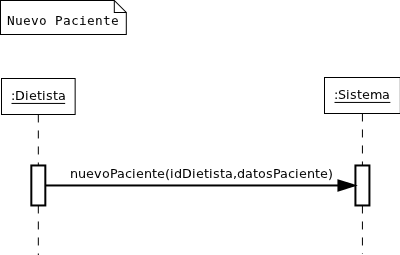
\includegraphics[scale=0.7]{../img/DS_NuevoPaciente.png}
  \end{center}
  \caption{Diagrama de secuencia: Nuevo Paciente}
\end{figure}
\textbf{Contrato de la operación:} nuevoPaciente(idDietista,datosPaciente)
\begin{itemize}
\item \textbf{Responsabilidades:} Registrar un nuevo paciente de un dietista en el sistema.
\item \textbf{Referencias cruzadas:} Caso de uso ``Nuevo Paciente''.
\item \textbf{Precondición:}
\begin{itemize}
\item Existe un dietista con id = idDietista en uso del sistema.
\item El paciente no existe en el sistema.
\item datosPaciente es válido.
\end{itemize}
\item \textbf{Postcondición:}
\begin{itemize}
\item El paciente se guarda en el sistema.
\end{itemize}
\end{itemize}

\textbf{Caso de Uso: Abrir Perfil Paciente}
\begin{itemize}
\item \textbf{Descripción:} Abrir perfil de un paciente en el sistema.
\item \textbf{Precondición:} El dietista y el paciente existen en el sistema.
\item \textbf{Postcondición:} El perfil del paciente se abre en el sistema.
\item \textbf{Actores:} Dietista(principal)
\item \textbf{Resumen:} El dietista desea abrir un perfil de un paciente en el sistema.
\item \textbf{Escenario Principal:}
\begin{enumerate}
\item El dietista solicita al sistema abrir un perfil de un paciente.
\item El sistema muestra el listado de pacientes existente, pertenecientes al dietista que lo solicita.
\item El dietista selecciona el perfil del paciente a abrir.
\item Se abre el perfil del paciente en el sistema.
\end{enumerate}
\item \textbf{Escenario Alternativo:}
\begin{enumerate}
\item[0] En cualquier momento el dietista puede cancelar el proceso.
\end{enumerate}
\end{itemize}
\begin{figure}[H]
  \label{ds_abrirpaciente}
  \begin{center}
    % Comentar si no está el paquete tkiz instalado, y descomentar la
    % linea siguiente. Comentar además la inclusión del paquete en
    % estilos/estiloBase.sty
    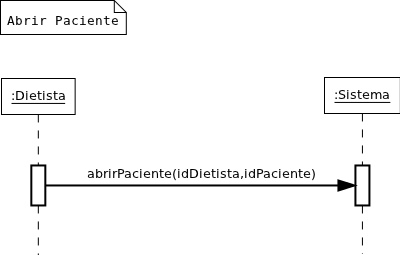
\includegraphics[scale=0.7]{../img/DS_AbrirPaciente.png}
  \end{center}
  \caption{Diagrama de secuencia: Abrir Perfil Paciente}
\end{figure}
\textbf{Contrato de la operación:} abrirPaciente(idDietista,idPaciente)
\begin{itemize}
\item \textbf{Responsabilidades:} Abrir un perfil de un paciente del dietista en el sistema.
\item \textbf{Referencias cruzadas:} Caso de uso ``Abrir Perfil Paciente''.
\item \textbf{Precondición:}
\begin{itemize}
\item El dietista con id = idDietista tiene su perfil abierto.
\item Existe un paciente con id = idPaciente.
\end{itemize}
\item \textbf{Postcondición:}
\begin{itemize}
\item El paciente con idPaciente se abre en el sistema.
\end{itemize}
\end{itemize}


\textbf{Caso de Uso: Editar Perfil Paciente}
\begin{itemize}
\item \textbf{Descripción:} Editar perfil de un paciente del sistema.
\item \textbf{Precondición:} El dietista y el paciente existen en el sistema.
\item \textbf{Postcondición:} El perfil del paciente se edita en el sistema.
\item \textbf{Actores:} Dietista(principal)
\item \textbf{Resumen:} El dietista desea editar el perfil de un paciente del sistema.
\item \textbf{Escenario Principal:}
\begin{enumerate}
\item El dietista solicita al sistema editar el perfil de un paciente.
\item El dietista presiona el botón guardar.
\item El sistema guarda los nuevos datos.
\end{enumerate}
\item \textbf{Escenario Alternativo:}
\begin{enumerate}
\item[2] El dietista no presiona el botón, los datos nuevos se perderán.
\end{enumerate}
\end{itemize}
\begin{figure}[H]
  \label{ds_editarpaciente}
  \begin{center}
    % Comentar si no está el paquete tkiz instalado, y descomentar la
    % linea siguiente. Comentar además la inclusión del paquete en
    % estilos/estiloBase.sty
    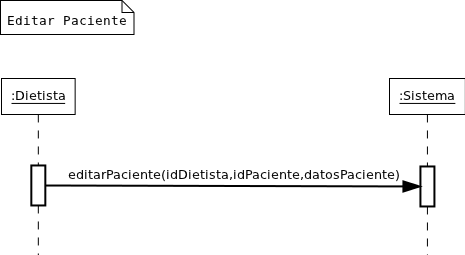
\includegraphics[scale=0.7]{../img/DS_EditarPaciente.png}
  \end{center}
  \caption{Diagrama de secuencia: Editar Datos Paciente}
\end{figure}
\textbf{Contrato de la operación:} editarPaciente(idDietista,idPaciente,datosPaciente)
\begin{itemize}
\item \textbf{Responsabilidades:} Editar el perfil de un paciente del dietista en el sistema.
\item \textbf{Referencias cruzadas:} Caso de uso ``Editar Perfil Paciente''.
\item \textbf{Precondición:}
\begin{itemize}
\item El dietista con id = idDietista tiene su perfil abierto.
\item El paciente con id = idPaciente tiene su perfil abierto.
\item datosPaciente es válido.
\end{itemize}
\item \textbf{Postcondición:}
\begin{itemize}
\item El paciente se edita en el sistema.
\end{itemize}
\end{itemize}

\textbf{Caso de Uso: Cerrar Perfil Paciente}
\begin{itemize}
\item \textbf{Descripción:} Cerrar perfil de paciente del sistema.
\item \textbf{Precondición:} El dietista y el paciente existen en el sistema.
\item \textbf{Postcondición:} El perfil del paciente se abre en el sistema.
\item \textbf{Actores:} Dietista(principal)
\item \textbf{Resumen:} El dietista desea cerrar el perfil de un paciente del sistema.
\item \textbf{Escenario Principal:}
\begin{enumerate}
\item El dietista solicita al sistema cerrar un perfil de un paciente.
\item El sistema solicita confirmación.
\item El dietista da la confirmación al cierre del perfil.
\item Se cierra el perfil del paciente en el sistema.
\end{enumerate}
\item \textbf{Escenario Alternativo:}
\begin{enumerate}
\item[0] En cualquier momento el dietista puede cancelar el proceso.
\item[3] El dietista no da la confirmación.
\item[3a] Se cancela el proceso.
\end{enumerate}
\end{itemize}
\begin{figure}[H]
  \label{ds_cerrarpaciente}
  \begin{center}
    % Comentar si no está el paquete tkiz instalado, y descomentar la
    % linea siguiente. Comentar además la inclusión del paquete en
    % estilos/estiloBase.sty
    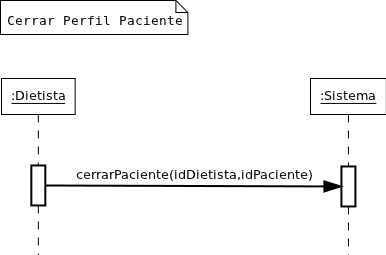
\includegraphics[scale=0.7]{../img/DS_CerrarPaciente.png}
  \end{center}
  \caption{Diagrama de secuencia: Cerrar Perfil Paciente}
\end{figure}
\textbf{Contrato de la operación:} cerrarPaciente(idDietista,idPaciente)
\begin{itemize}
\item \textbf{Responsabilidades:} Cerrar el perfil de un paciente del dietista en el sistema.
\item \textbf{Referencias cruzadas:} Caso de uso ``Cerrar Perfil Paciente''.
\item \textbf{Precondición:}
\begin{itemize}
\item El dietista con id = idDietista tiene su perfil abierto.
\item El paciente con id = idPaciente tiene su perfil abierto.
\end{itemize}
\item \textbf{Postcondición:}
\begin{itemize}
\item El paciente se cierra en el sistema.
\end{itemize}
\end{itemize}



\textbf{Caso de Uso: Eliminar Perfil Paciente}
\begin{itemize}
\item \textbf{Descripción:} Eliminar perfil de paciente del sistema.
\item \textbf{Precondición:} El dietista y el paciente existen en el sistema.
\item \textbf{Postcondición:} El paciente se elimina del sistema.
\item \textbf{Actores:} Dietista(principal)
\item \textbf{Resumen:} El dietista desea eliminar el perfil de un paciente del sistema.
\item \textbf{Escenario Principal:}
\begin{enumerate}
\item El dietista solicita al sistema eliminar un perfil de un paciente.
\item El sistema muestra un listado de los pacientes pertenecientes al dietista en uso.
\item El dietista selecciona el perfil que quiere eliminar.
\item El sistema elimina el perfil de paciente seleccionado.
\end{enumerate}
\item \textbf{Escenario Alternativo:}
\begin{enumerate}
\item[0] En cualquier momento el dietista puede cancelar el proceso.
\end{enumerate}
\end{itemize}
\begin{figure}[H]
  \label{ds_eliminarpaciente}
  \begin{center}
    % Comentar si no está el paquete tkiz instalado, y descomentar la
    % linea siguiente. Comentar además la inclusión del paquete en
    % estilos/estiloBase.sty
    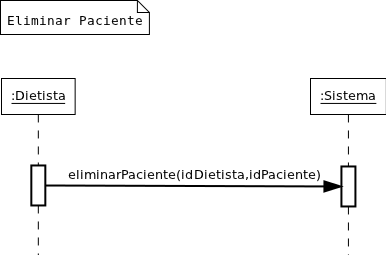
\includegraphics[scale=0.7]{../img/DS_EliminarPaciente.png}
  \end{center}
  \caption{Diagrama de secuencia: Eliminar Paciente}
\end{figure}
\textbf{Contrato de la operación:} eliminarPaciente(idDietista,idPaciente)
\begin{itemize}
\item \textbf{Responsabilidades:} Eliminar el perfil de un paciente del dietista en el sistema.
\item \textbf{Referencias cruzadas:} Caso de uso ``Eliminar Perfil Paciente''.
\item \textbf{Precondición:}
\begin{itemize}
\item El dietista con id = idDietista tiene su perfil abierto.
\item El paciente con id = idPaciente existe.
\end{itemize}
\item \textbf{Postcondición:}
\begin{itemize}
\item El paciente con idPaciente se elimina del sistema.
\end{itemize}
\end{itemize}

\textbf{Caso de Uso: Añadir Información Médica}
\begin{itemize}
\item \textbf{Descripción:} Añadir información médica a un paciente del sistema.
\item \textbf{Precondición:} El dietista y el paciente existen en el sistema.
\item \textbf{Postcondición:} Se añade la información médica al paciente del sistema.
\item \textbf{Actores:} Dietista(principal)
\item \textbf{Resumen:} El dietista desea añadir información médica a un paciente del sistema.
\item \textbf{Escenario Principal:}
\begin{enumerate}
\item El dietista solicita al sistema añadir información médica a un paciente.
\item El dietista introduce los campos solicitados.
\item El sistema almacena los datos en el sistema.
\end{enumerate}
\item \textbf{Escenario Alternativo:}
\begin{enumerate}
\item[0] En cualquier momento el dietista puede cancelar el proceso.
\end{enumerate}
\end{itemize}
\begin{figure}[H]
  \label{ds_anadirinfomed}
  \begin{center}
    % Comentar si no está el paquete tkiz instalado, y descomentar la
    % linea siguiente. Comentar además la inclusión del paquete en
    % estilos/estiloBase.sty
    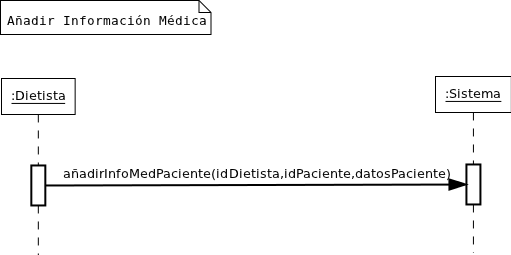
\includegraphics[scale=0.7]{../img/DS_AnadirInfoMed.png}
  \end{center}
  \caption{Diagrama de secuencia: Añadir Información Médica}
\end{figure}
\textbf{Contrato de la operación:} añadirInfoMedPaciente(idDietista,idPaciente,datosPaciente)
\begin{itemize}
\item \textbf{Responsabilidades:} Añadir información médica a un paciente del dietista en el sistema.
\item \textbf{Referencias cruzadas:} Caso de uso ``Añadir Información Médica''.
\item \textbf{Precondición:}
\begin{itemize}
\item El dietista con id = idDietista tiene su perfil abierto.
\item El paciente con id = idPaciente tiene su perfil abierto.
\item datosPaciente es válido.
\end{itemize}
\item \textbf{Postcondición:}
\begin{itemize}
\item Se añade la información médica al paciente en el sistema.
\end{itemize}
\end{itemize}

\textbf{Caso de Uso: Modificar Información Médica}
\begin{itemize}
\item \textbf{Descripción:} Modificar la información médica de un paciente del sistema.
\item \textbf{Precondición:} El dietista y el paciente existen en el sistema.
\item \textbf{Postcondición:} Se modifica la información médica al paciente del sistema.
\item \textbf{Actores:} Dietista(principal)
\item \textbf{Resumen:} El dietista desea modificar la información médica de un paciente del sistema.
\item \textbf{Escenario Principal:}
\begin{enumerate}
\item El dietista solicita al sistema modificar la información médica de un paciente.
\item El dietista introduce los campos solicitados.
\item El sistema almacena los datos en el sistema.
\end{enumerate}
\item \textbf{Escenario Alternativo:}
\begin{enumerate}
\item[0] En cualquier momento el dietista puede cancelar el proceso.
\end{enumerate}
\end{itemize}
\begin{figure}[H]
  \label{ds_modificarinfomed}
  \begin{center}
    % Comentar si no está el paquete tkiz instalado, y descomentar la
    % linea siguiente. Comentar además la inclusión del paquete en
    % estilos/estiloBase.sty
    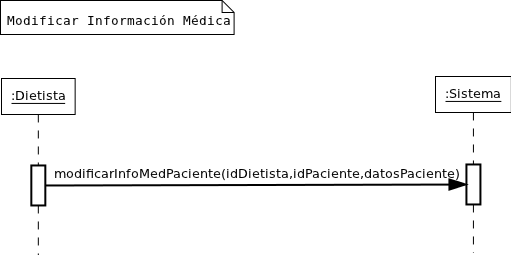
\includegraphics[scale=0.7]{../img/DS_ModificarInfoMed.png}
  \end{center}
  \caption{Diagrama de secuencia: Modificar Información Médica}
\end{figure}
\textbf{Contrato de la operación:} modificarInfoMedPaciente(idDietista,idPaciente,datosPaciente)
\begin{itemize}
\item \textbf{Responsabilidades:} Modificar información médica de un paciente del dietista en el sistema.
\item \textbf{Referencias cruzadas:} Caso de uso ``Modificar Información Médica''.
\item \textbf{Precondición:}
\begin{itemize}
\item El dietista con id = idDietista tiene su perfil abierto.
\item El paciente con id = idPaciente tiene su perfil abierto.
\item datosPaciente es válido.
\end{itemize}
\item \textbf{Postcondición:}
\begin{itemize}
\item Se modifica la información médica del paciente en el sistema.
\end{itemize}
\end{itemize}


\textbf{Caso de Uso: Añadir Información General}
\begin{itemize}
\item \textbf{Descripción:} Añadir información general a un paciente del sistema.
\item \textbf{Precondición:} El dietista y el paciente existen en el sistema.
\item \textbf{Postcondición:} Se añade la información general del paciente del sistema.
\item \textbf{Actores:} Dietista(principal) y Paciente(secundario)
\item \textbf{Resumen:} El dietista desea añadir información general a un paciente del sistema.
\item \textbf{Escenario Principal:}
\begin{enumerate}
\item El dietista solicita al sistema añadir información general a un paciente.
\item El dietista introduce los campos solicitados.
\item El sistema almacena los datos en el sistema.
\end{enumerate}
\item \textbf{Escenario Alternativo:}
\begin{enumerate}
\item[0] En cualquier momento el dietista puede cancelar el proceso.
\end{enumerate}
\end{itemize}
\begin{figure}[H]
  \label{ds_anadirinfogen}
  \begin{center}
    % Comentar si no está el paquete tkiz instalado, y descomentar la
    % linea siguiente. Comentar además la inclusión del paquete en
    % estilos/estiloBase.sty
    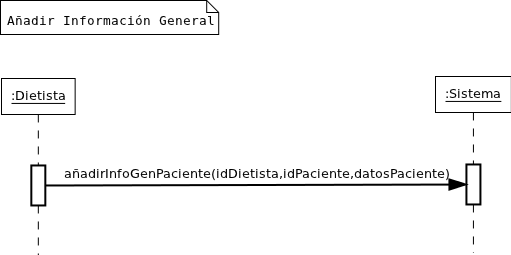
\includegraphics[scale=0.7]{../img/DS_AnadirInfoGen.png}
  \end{center}
  \caption{Diagrama de secuencia: Añadir Información General}
\end{figure}
\textbf{Contrato de la operación:} añadirInfoGenPaciente(idDietista,idPaciente,datosPaciente)
\begin{itemize}
\item \textbf{Responsabilidades:} Añadir información general a un paciente del dietista en el sistema.
\item \textbf{Referencias cruzadas:} Caso de uso ``Añadir Información General''.
\item \textbf{Precondición:}
\begin{itemize}
\item El dietista con id = idDietista tiene su perfil abierto.
\item El paciente con id = idPaciente tiene su perfil abierto.
\item datosPaciente es válido.
\end{itemize}
\item \textbf{Postcondición:}
\begin{itemize}
\item Se añade la información general al paciente en el sistema.
\end{itemize}
\end{itemize}

\textbf{Caso de Uso: Añadir Diario Dietético}
\begin{itemize}
\item \textbf{Descripción:} Añadir un diario dietético a un paciente del sistema.
\item \textbf{Precondición:} El dietista y el paciente existen en el sistema.
\item \textbf{Postcondición:} Se añade el diario dietético al paciente del sistema.
\item \textbf{Actores:} Dietista(principal) y Paciente(secundario)
\item \textbf{Resumen:} El dietista desea añadir un diario dietético a un paciente del sistema.
\item \textbf{Escenario Principal:}
\begin{enumerate}
\item El dietista solicita al sistema añadir un diario dietético a un paciente.
\item El dietista introduce los campos solicitados.
\item El sistema almacena los datos en el sistema.
\end{enumerate}
\item \textbf{Escenario Alternativo:}
\begin{enumerate}
\item[0] En cualquier momento el dietista puede cancelar el proceso.
\end{enumerate}
\end{itemize}
\begin{figure}[H]
  \label{ds_anadirdiariodiet}
  \begin{center}
    % Comentar si no está el paquete tkiz instalado, y descomentar la
    % linea siguiente. Comentar además la inclusión del paquete en
    % estilos/estiloBase.sty
    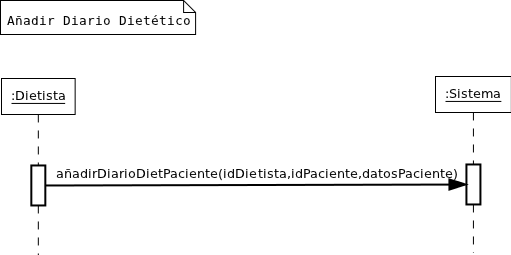
\includegraphics[scale=0.7]{../img/DS_AnadirDiarioDiet.png}
  \end{center}
  \caption{Diagrama de secuencia: Añadir Diario Dietético}
\end{figure}
\textbf{Contrato de la operación:} añadirDiarioDietPaciente(idDietista,idPaciente,datosPaciente)
\begin{itemize}
\item \textbf{Responsabilidades:} Añadir un diario dietético a un paciente del dietista en el sistema.
\item \textbf{Referencias cruzadas:} Caso de uso ``Añadir Diario Dietético''.
\item \textbf{Precondición:}
\begin{itemize}
\item El dietista con id = idDietista tiene su perfil abierto.
\item El paciente con id = idPaciente tiene su perfil abierto.
\item datosPaciente es válido.
\end{itemize}
\item \textbf{Postcondición:}
\begin{itemize}
\item Se añade el diario dietético al paciente en el sistema.
\end{itemize}
\end{itemize}


\textbf{Caso de Uso: Eliminar Diario Dietético}
\begin{itemize}
\item \textbf{Descripción:} Eliminar un diario dietético de un paciente del sistema.
\item \textbf{Precondición:} El dietista y el paciente existen en el sistema.
\item \textbf{Postcondición:} Se elimina el diario dietético del paciente del sistema.
\item \textbf{Actores:} Dietista(principal)
\item \textbf{Resumen:} El dietista desea eliminar un diario dietético de un paciente del sistema.
\item \textbf{Escenario Principal:}
\begin{enumerate}
\item El dietista solicita al sistema eliminar un diario dietético de un paciente.
\item El dietista selecciona el diario dietético a eliminar.
\item El sistema elimina el diario dietético del sistema.
\end{enumerate}
\item \textbf{Escenario Alternativo:}
\begin{enumerate}
\item[0] En cualquier momento el dietista puede cancelar el proceso.
\end{enumerate}
\end{itemize}
\begin{figure}[H]
  \label{ds_eliminardiariodiet}
  \begin{center}
    % Comentar si no está el paquete tkiz instalado, y descomentar la
    % linea siguiente. Comentar además la inclusión del paquete en
    % estilos/estiloBase.sty
    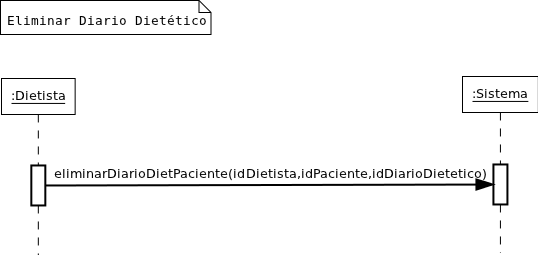
\includegraphics[scale=0.7]{../img/DS_EliminarDiarioDiet.png}
  \end{center}
  \caption{Diagrama de secuencia: Eliminar Diario Dietético}
\end{figure}
\textbf{Contrato de la operación:} eliminarDiarioDietPaciente(idDietista,idPaciente,idDiarioDietetico)
\begin{itemize}
\item \textbf{Responsabilidades:} Eliminar un diario dietético de un paciente del dietista en el sistema.
\item \textbf{Referencias cruzadas:} Caso de uso ``Eliminar Diario Dietético''.
\item \textbf{Precondición:}
\begin{itemize}
\item El dietista con id = idDietista tiene su perfil abierto.
\item El paciente con id = idPaciente tiene su perfil abierto.
\item Existe un diario dietético con id = idDiarioDietetico.
\end{itemize}
\item \textbf{Postcondición:}
\begin{itemize}
\item Se elimina el diario dietético del paciente en el sistema.
\end{itemize}
\end{itemize}


\textbf{Caso de Uso: Añadir Recordatorio}
\begin{itemize}
\item \textbf{Descripción:} Añadir un recordatorio 24h a un paciente del sistema.
\item \textbf{Precondición:} El dietista y el paciente existen en el sistema.
\item \textbf{Postcondición:} Se añade el recordatorio 24h al paciente del sistema.
\item \textbf{Actores:} Dietista(principal) y Paciente(secundario)
\item \textbf{Resumen:} El dietista desea añadir un recordatorio 24h a un paciente del sistema.
\item \textbf{Escenario Principal:}
\begin{enumerate}
\item El dietista solicita al sistema añadir un recordatorio 24h a un paciente.
\item El dietista introduce los campos solicitados.
\item El sistema almacena los datos en el sistema.
\end{enumerate}
\item \textbf{Escenario Alternativo:}
\begin{enumerate}
\item[0] En cualquier momento el dietista puede cancelar el proceso.
\end{enumerate}
\end{itemize}
\begin{figure}[H]
  \label{ds_anadirrecordatorio}
  \begin{center}
    % Comentar si no está el paquete tkiz instalado, y descomentar la
    % linea siguiente. Comentar además la inclusión del paquete en
    % estilos/estiloBase.sty
    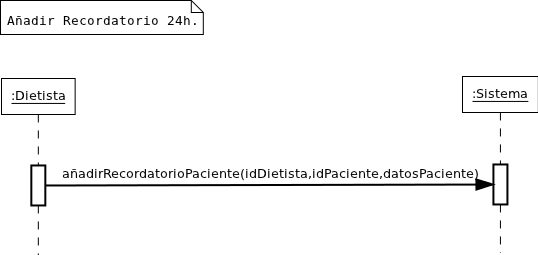
\includegraphics[scale=0.7]{../img/DS_AnadirRecordatorio.png}
  \end{center}
  \caption{Diagrama de secuencia: Añadir Recordatorio 24h}
\end{figure}
\textbf{Contrato de la operación:} añadirRecordatorioPaciente(idDietista,idPaciente,datosPaciente)
\begin{itemize}
\item \textbf{Responsabilidades:} Añadir un recordatorio 24h a un paciente del dietista en el sistema.
\item \textbf{Referencias cruzadas:} Caso de uso ``Añadir Recordatorio''.
\item \textbf{Precondición:}
\begin{itemize}
\item El dietista con id = idDietista tiene su perfil abierto.
\item El paciente con id = idPaciente tiene su perfil abierto.
\item datosPaciente es válido.
\end{itemize}
\item \textbf{Postcondición:}
\begin{itemize}
\item Se añade el recordatorio 24h al paciente en el sistema.
\end{itemize}
\end{itemize}


\textbf{Caso de Uso: Eliminar Recordatorio}
\begin{itemize}
\item \textbf{Descripción:} Eliminar un recordatorio 24h de un paciente del sistema.
\item \textbf{Precondición:} El dietista y el paciente existen en el sistema.
\item \textbf{Postcondición:} Se elimina el recordatorio 24h del paciente del sistema.
\item \textbf{Actores:} Dietista(principal)
\item \textbf{Resumen:} El dietista desea eliminar un recordatorio 24h de un paciente del sistema.
\item \textbf{Escenario Principal:}
\begin{enumerate}
\item El dietista solicita al sistema eliminar un recordatorio 24h de un paciente.
\item El dietista selecciona el recordatorio 24h a eliminar.
\item El sistema elimina el recordatorio 24h del sistema.
\end{enumerate}
\item \textbf{Escenario Alternativo:}
\begin{enumerate}
\item[0] En cualquier momento el dietista puede cancelar el proceso.
\end{enumerate}
\end{itemize}
\begin{figure}[H]
  \label{ds_eliminarrecordatorio}
  \begin{center}
    % Comentar si no está el paquete tkiz instalado, y descomentar la
    % linea siguiente. Comentar además la inclusión del paquete en
    % estilos/estiloBase.sty
    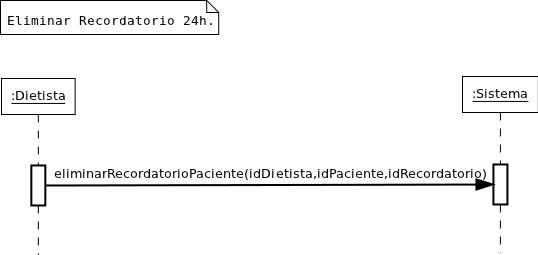
\includegraphics[scale=0.7]{../img/DS_EliminarRecordatorio.png}
  \end{center}
  \caption{Diagrama de secuencia: Eliminar Recordatorio 24h.}
\end{figure}
\textbf{Contrato de la operación:} eliminarRecordatorioPaciente(idDietista,idPaciente,idRecordatorio)
\begin{itemize}
\item \textbf{Responsabilidades:} Eliminar un recordatorio 24h de un paciente del dietista en el sistema.
\item \textbf{Referencias cruzadas:} Caso de uso ``Eliminar Recordatorio''.
\item \textbf{Precondición:}
\begin{itemize}
\item El dietista con id = idDietista tiene su perfil abierto.
\item El paciente con id = idPaciente tiene su perfil abierto.
\item Existe un recordatorio 24h con id = idRecordatorio.
\end{itemize}
\item \textbf{Postcondición:}
\begin{itemize}
\item Se elimina el recordatorio 24h del paciente en el sistema.
\end{itemize}
\end{itemize}

\textbf{Caso de Uso: Añadir Frecuencia de Ingesta}
\begin{itemize}
\item \textbf{Descripción:} Añadir la frecuencia de ingesta de alimentos de un paciente del sistema.
\item \textbf{Precondición:} El dietista y el paciente existen en el sistema.
\item \textbf{Postcondición:} Se añade la frecuencia de ingesta de alimentos al paciente del sistema.
\item \textbf{Actores:} Dietista(principal) y Paciente(secundario)
\item \textbf{Resumen:} El dietista desea añadir la frecuencia de ingesta de alimentos a un paciente del sistema.
\item \textbf{Escenario Principal:}
\begin{enumerate}
\item El dietista solicita al sistema añadir la frecuencia de ingesta de alimentos a un paciente.
\item El dietista introduce los campos solicitados.
\item El sistema almacena los datos en el sistema.
\end{enumerate}
\item \textbf{Escenario Alternativo:}
\begin{enumerate}
\item[0] En cualquier momento el dietista puede cancelar el proceso.
\end{enumerate}
\end{itemize}
\begin{figure}[H]
  \label{ds_anadirfrecing}
  \begin{center}
    % Comentar si no está el paquete tkiz instalado, y descomentar la
    % linea siguiente. Comentar además la inclusión del paquete en
    % estilos/estiloBase.sty
    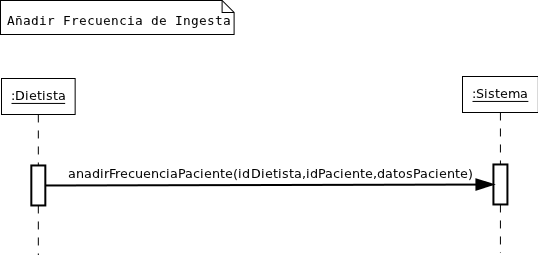
\includegraphics[scale=0.7]{../img/DS_AnadirFrecIng.png}
  \end{center}
  \caption{Diagrama de secuencia: Añadir Frecuencia de Ingesta}
\end{figure}
\textbf{Contrato de la operación:} añadirFrecuenciaPaciente(idDietista,idPaciente,datosPaciente)
\begin{itemize}
\item \textbf{Responsabilidades:} Añadir la frecuencia de ingesta de alimentos a un paciente del dietista en el sistema.
\item \textbf{Referencias cruzadas:} Caso de uso ``Añadir Frecuencia de Ingesta''.
\item \textbf{Precondición:}
\begin{itemize}
\item El dietista con id = idDietista tiene su perfil abierto.
\item El paciente con id = idPaciente tiene su perfil abierto.
\item datosPaciente es válido.
\end{itemize}
\item \textbf{Postcondición:}
\begin{itemize}
\item Se añade la frecuencia de ingesta de alimentos al paciente en el sistema.
\end{itemize}
\end{itemize}


\textbf{Caso de Uso: Añadir Recetas a Semanario}
\begin{itemize}
\item \textbf{Descripción:} Añadir una receta al semanario de un paciente del sistema.
\item \textbf{Precondición:} El dietista y el paciente existen en el sistema.
\item \textbf{Postcondición:} Se añade una receta al semanario del paciente del sistema.
\item \textbf{Actores:} Dietista(principal)
\item \textbf{Resumen:} El dietista desea añadir una receta al semanario de un paciente del sistema.
\item \textbf{Escenario Principal:}
\begin{enumerate}
\item El dietista solicita al sistema añadir una receta al semanario de un paciente.
\item El dietista selecciona la receta a añadir.
\item El sistema registra los datos en el sistema.
\end{enumerate}
\item \textbf{Escenario Alternativo:}
\begin{enumerate}
\item[0] En cualquier momento el dietista puede cancelar el proceso.
\end{enumerate}
\end{itemize}
\begin{figure}[H]
  \label{ds_anadirrecetasemanario}
  \begin{center}
    % Comentar si no está el paquete tkiz instalado, y descomentar la
    % linea siguiente. Comentar además la inclusión del paquete en
    % estilos/estiloBase.sty
    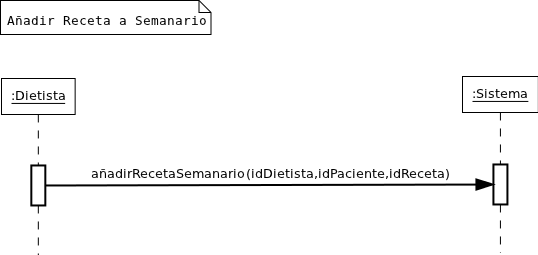
\includegraphics[scale=0.7]{../img/DS_AnadirRecetaSemanario.png}
  \end{center}
  \caption{Diagrama de secuencia: Añadir Receta a Semanario}
\end{figure}
\textbf{Contrato de la operación:} añadirRecetaSemanario(idDietista,idPaciente,idReceta)
\begin{itemize}
\item \textbf{Responsabilidades:} Añadir una receta al semanario de un paciente del dietista en el sistema.
\item \textbf{Referencias cruzadas:} Caso de uso ``Añadir Receta a Semanario''.
\item \textbf{Precondición:}
\begin{itemize}
\item El dietista con id = idDietista tiene su perfil abierto.
\item El paciente con id = idPaciente tiene su perfil abierto.
\item Existe una receta con id = idReceta.
\end{itemize}
\item \textbf{Postcondición:}
\begin{itemize}
\item Se añade la receta al semanario del paciente en el sistema.
\end{itemize}
\end{itemize}


\textbf{Caso de Uso: Ver Semanarios}
\begin{itemize}
\item \textbf{Descripción:} Ver semanarios de un paciente del sistema.
\item \textbf{Precondición:} El dietista y el paciente existen en el sistema.
\item \textbf{Postcondición:} Ninguna.
\item \textbf{Actores:} Dietista(principal)
\item \textbf{Resumen:} El dietista desea ver los semanarios de un paciente del sistema.
\item \textbf{Escenario Principal:}
\begin{enumerate}
\item El dietista solicita al sistema ver los semanarios de un paciente.
\item El sistema muestra los datos en el sistema.
\end{enumerate}
\item \textbf{Escenario Alternativo:}
\begin{enumerate}
\item[0] En cualquier momento el dietista puede cancelar el proceso.
\item[2] No hay ningún semanario registrado del paciente. El sistema no mostrará nada.
\end{enumerate}
\end{itemize}
\begin{figure}[H]
  \label{ds_versemanarios}
  \begin{center}
    % Comentar si no está el paquete tkiz instalado, y descomentar la
    % linea siguiente. Comentar además la inclusión del paquete en
    % estilos/estiloBase.sty
    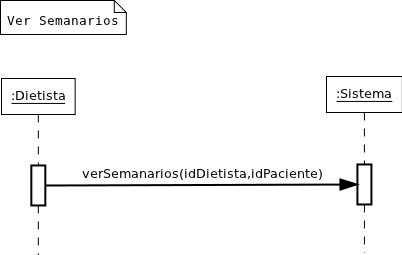
\includegraphics[scale=0.7]{../img/DS_VerSemanarios.png}
  \end{center}
  \caption{Diagrama de secuencia: Ver Semanarios de un Paciente}
\end{figure}
\textbf{Contrato de la operación:} verSemanarios(idDietista,idPaciente)
\begin{itemize}
\item \textbf{Responsabilidades:} Ver los semanarios de un paciente del dietista en el sistema.
\item \textbf{Referencias cruzadas:} Caso de uso ``Ver Semanarios''.
\item \textbf{Precondición:}
\begin{itemize}
\item El dietista con id = idDietista tiene su perfil abierto.
\item El paciente con id = idPaciente tiene su perfil abierto.
\end{itemize}
\item \textbf{Postcondición:}
\begin{itemize}
\item El sistema muestra los semanarios del paciente del sistema.
\end{itemize}
\end{itemize}

\newpage
\subsubsection{Casos de uso respecto a la gestión de recetas}

\begin{figure}[H]
  \label{cu_receta}
  \begin{center}
    % Comentar si no está el paquete tkiz instalado, y descomentar la
    % linea siguiente. Comentar además la inclusión del paquete en
    % estilos/estiloBase.sty
    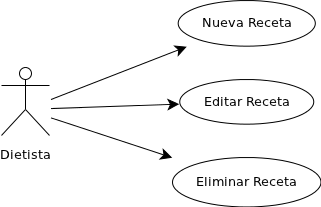
\includegraphics[scale=0.5]{../img/CU_Receta.png}
  \end{center}
  \caption{Diagrama de caso de uso: Gestión de recetas}
\end{figure}

\textbf{Caso de Uso: Nueva Receta}
\begin{itemize}
\item \textbf{Descripción:} Añadir una nueva receta en el sistema.
\item \textbf{Precondición:} Hay un dietista en uso y la receta no existe.
\item \textbf{Postcondición:} La receta del dietista se registra en el sistema.
\item \textbf{Actores:} Dietista(principal)
\item \textbf{Resumen:} El dietista desea registrar una nueva receta en el sistema.
\item \textbf{Escenario Principal:}
\begin{enumerate}
\item El dietista solicita al sistema registrar una nueva receta.
\item El dietista rellena los campos solicitados para la receta.
\item El sistema comprueba los datos.
\item El sistema almacena los datos.
\end{enumerate}
\item \textbf{Escenario Alternativo:}
\begin{enumerate}
\item[0] El dietista puede cancelar el proceso en cualquier momento.
\item[3] La receta ya existe en el sistema. Mensaje de advertencia del sistema.
\end{enumerate}
\end{itemize}
\begin{figure}[H]
  \label{ds_nuevareceta}
  \begin{center}
    % Comentar si no está el paquete tkiz instalado, y descomentar la
    % linea siguiente. Comentar además la inclusión del paquete en
    % estilos/estiloBase.sty
    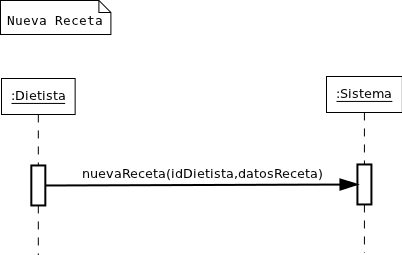
\includegraphics[scale=0.7]{../img/DS_NuevaReceta.png}
  \end{center}
  \caption{Diagrama de secuencia: Nueva Receta}
\end{figure}
\textbf{Contrato de la operación:} nuevaReceta(idDietista, datosReceta)
\begin{itemize}
\item \textbf{Responsabilidades:} Registrar una nueva receta en el sistema.
\item \textbf{Referencias cruzadas:} Caso de uso ``Nueva Receta''.
\item \textbf{Precondición:}
\begin{itemize}
\item Existe un dietista con id = idDietista en uso.
\item datosReceta es válido.
\end{itemize}
\item \textbf{Postcondición:}
\begin{itemize}
\item La receta se guarda en el sistema.
\end{itemize}
\end{itemize}

\textbf{Caso de Uso: Editar Receta}
\begin{itemize}
\item \textbf{Descripción:} Editar una receta del sistema.
\item \textbf{Precondición:} Hay un dietista en uso y la receta existe.
\item \textbf{Postcondición:} La receta del dietista se registra en el sistema con los nuevos datos.
\item \textbf{Actores:} Dietista(principal)
\item \textbf{Resumen:} El dietista desea editar una receta del sistema.
\item \textbf{Escenario Principal:}
\begin{enumerate}
\item El dietista solicita al sistema editar una receta.
\item El sistema muestra el listado de recetas.
\item El dietista selecciona la receta a editar.
\item El dietista rellena los campos que desea cambiar para la receta.
\item El sistema almacena los nuevos datos.
\end{enumerate}
\item \textbf{Escenario Alternativo:}
\begin{enumerate}
\item[0] El dietista puede cancelar el proceso en cualquier momento.
\end{enumerate}
\end{itemize}
\begin{figure}[H]
  \label{ds_editarreceta}
  \begin{center}
    % Comentar si no está el paquete tkiz instalado, y descomentar la
    % linea siguiente. Comentar además la inclusión del paquete en
    % estilos/estiloBase.sty
    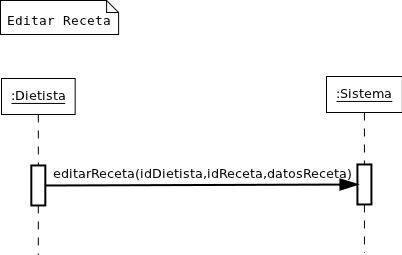
\includegraphics[scale=0.7]{../img/DS_EditarReceta.png}
  \end{center}
  \caption{Diagrama de secuencia: Editar Receta}
\end{figure}
\textbf{Contrato de la operación:} editarReceta(idDietista, idReceta, datosReceta)
\begin{itemize}
\item \textbf{Responsabilidades:} Editar una receta del sistema.
\item \textbf{Referencias cruzadas:} Caso de uso ``Editar Receta''.
\item \textbf{Precondición:}
\begin{itemize}
\item Existe un dietista con id = idDietista en uso.
\item Existe una receta con id = idReceta.
\item datosReceta es válido.
\end{itemize}
\item \textbf{Postcondición:}
\begin{itemize}
\item La receta se guarda con los nuevos datos en el sistema.
\end{itemize}
\end{itemize}

\textbf{Caso de Uso: Eliminar Receta}
\begin{itemize}
\item \textbf{Descripción:} Eliminar una receta del sistema.
\item \textbf{Precondición:} Hay un dietista en uso y la receta existe.
\item \textbf{Postcondición:} La receta del dietista se elimina del sistema.
\item \textbf{Actores:} Dietista(principal)
\item \textbf{Resumen:} El dietista desea eliminar una receta del sistema.
\item \textbf{Escenario Principal:}
\begin{enumerate}
\item El dietista solicita al sistema eliminar una receta.
\item El sistema muestra el listado de recetas.
\item El dietista selecciona la receta a eliminar.
\item El sistema elimina la receta del sistema.
\end{enumerate}
\item \textbf{Escenario Alternativo:}
\begin{enumerate}
\item[0] El dietista puede cancelar el proceso en cualquier momento.
\end{enumerate}
\end{itemize}
\begin{figure}[H]
  \label{ds_eliminarreceta}
  \begin{center}
    % Comentar si no está el paquete tkiz instalado, y descomentar la
    % linea siguiente. Comentar además la inclusión del paquete en
    % estilos/estiloBase.sty
    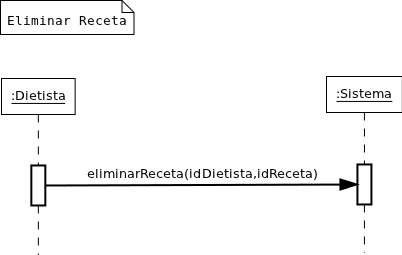
\includegraphics[scale=0.7]{../img/DS_EliminarReceta.png}
  \end{center}
  \caption{Diagrama de secuencia: Eliminar Receta}
\end{figure}
\textbf{Contrato de la operación:} eliminarReceta(idDietista, idReceta)
\begin{itemize}
\item \textbf{Responsabilidades:} Eliminar una receta del sistema.
\item \textbf{Referencias cruzadas:} Caso de uso ``Eliminar Receta''.
\item \textbf{Precondición:}
\begin{itemize}
\item Existe un dietista con id = idDietista en uso.
\item Existe una receta con id = idReceta.
\end{itemize}
\item \textbf{Postcondición:}
\begin{itemize}
\item La receta se elimina del sistema.
\end{itemize}
\end{itemize}

\subsection{Modelos conceptual de datos.}
\subsubsection{Diagrama conceptual de clases.}
\begin{figure}[H]
  \label{ds_eliminarreceta}
  \begin{center}
    % Comentar si no está el paquete tkiz instalado, y descomentar la
    % linea siguiente. Comentar además la inclusión del paquete en
    % estilos/estiloBase.sty
    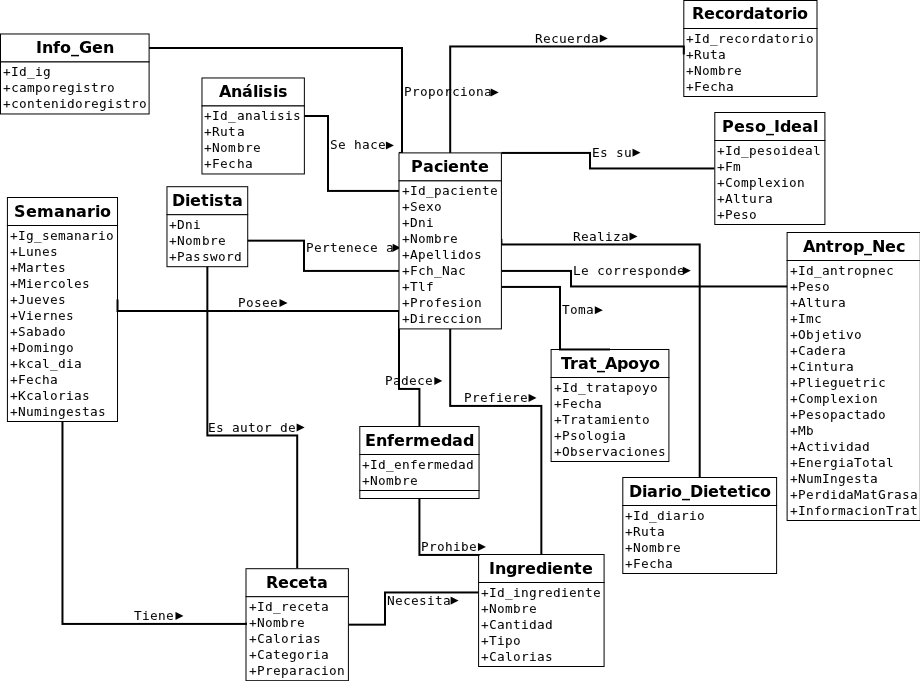
\includegraphics[scale=0.5]{../img/Diagrama_Clases.png}
  \end{center}
  \caption{Modelo conceptual de datos: Diagrama conceptual de clases}
\end{figure}
\subsubsection{Restricciones de clave primaria.}
\textbf{Clave primaria:}
(Dietista, d\_dni),
(Paciente, p\_id),
(Semanario, s\_id),
(Enfermedad, ep\_id),
(Receta, r\_id),
(Ingrediente, i\_id)
